% This is a (brief) model paper using the achemso class
% The document class accepts keyval options, which should include
% the target journal and optionally the manuscript type.

\documentclass[journal=langd5, manuscript=article, layout=twocolumn]{achemso}

% Place any additional packages needed here.  Only include packages
% which are essential, to avoid problems later. Do NOT use any
% packages which require e-TeX (for example etoolbox): the e-TeX
% extensions are not currently available on the ACS conversion
% servers.

\usepackage[version=3]{mhchem} % Formula subscripts using \ce{}
\usepackage[T1]{fontenc}       % Use modern font encodings
\usepackage{amsmath, amssymb, amsfonts}
\usepackage{graphicx, gensymb}

% If issues arise when submitting your manuscript, you may want to
% un-comment the next line.  This provides information on the
% version of every file you have used.
%\listfiles

% Place any additional macros here.  Please use \newcommand* where
% possible, and avoid layout-changing macros (which are not used
% when typesetting).

\SectionNumbersOn
\graphicspath{ {Figures/} }
\newcommand{\tdc}[3][]{\frac{\mathrm{d}^{#1}#2}{\mathrm{d}#3^{#1}}} % total differential change.
\newcommand{\pdc}[3][]{\frac{\partial^{#1} #2}{\partial #3^{#1}}} % partial differential change.
\newcommand{\td}[1]{\mathrm{d}#1}
\newcommand{\pd}[1]{\partial#1}

% Meta-data block
% ---------------
% Each author should be given as a separate \author command.
%
% Corresponding authors should have an e-mail given after the author
% name as an \email command. Phone and fax numbers can be given
% using \phone and \fax, respectively; this information is optional.
% The affiliation of authors is given after the authors; each
% \affiliation command applies to all preceding authors not already
% assigned an affiliation.
%
% The affiliation takes an option argument for the short name.  This
% will typically be something like "University of Somewhere".
% The \altaffiliation macro should be used for new address, etc.
% On the other hand, \alsoaffiliation is used on a per author basis
% when authors are associated with multiple institutions.

\author{V. S. Akella}
\affiliation{Collective Interactions Unit, OIST Graduate University, Okinawa, Japan 904-0495}
\author{D. K. Singh}
\affiliation{Collective Interactions Unit, OIST Graduate University, Okinawa, Japan 904-0495}
\author{R. K. Singh}
\affiliation{School of Engineering, Brown University, 182 Hope Street, Providence, RI 02906, USA}
\author{S. Mandre}
\affiliation{School of Engineering, Brown University, 182 Hope Street, Providence, RI 02906, USA}
\email{shreyas_mandre@brown.edu}
\author{M. M. Bandi}
\affiliation{Collective Interactions Unit, OIST Graduate University, Okinawa, Japan 904-0495}
\email{bandi@oist.jp}

% The document title should be given as usual. Some journals require
% a running title from the author: this should be supplied as an
% optional argument to \title.

\title[]{Dynamics of a Camphoric Acid boat at the air-water interface} 

% Some journals require a list of abbreviations or keywords to be
% supplied. These should be set up here, and will be printed after
% the title and author information, if needed.

\abbreviations{CA, DI}
\keywords{Marangoni flow, Self-propulsion}

% The manuscript does not need to include \maketitle, which is
% executed automatically.

\begin{document}

% The "tocentry" environment can be used to create an entry for the
% graphical table of contents. It is given here as some journals
% require that it is printed as part of the abstract page. It will
% be automatically moved as appropriate.

% \begin{tocentry}

% Some journals require a graphical entry for the Table of Contents.
% This should be laid out ``print ready'' so that the sizing of the
% text is correct.

% Inside the \texttt{tocentry} environment, the font used is Helvetica
% 8\,pt, as required by \emph{Journal of the American Chemical
% Society}.

% The surrounding frame is 9\,cm by 3.5\,cm, which is the maximum
% permitted for  \emph{Journal of the American Chemical Society}
% graphical table of content entries. The box will not resize if the
% content is too big: instead it will overflow the edge of the box.

% This box and the associated title will always be printed on a
% separate page at the end of the document.

% \end{tocentry}

% The abstract environment will automatically gobble the contents
% if an abstract is not used by the target journal.

\begin{abstract}
%We experimentally study the physics of camphoric acid loaded agarose gel tablets (cboats) at the air-water interface. Camphoric acid spreads over the air-water interface due to the interfacial tension forces. When a cboat is held fixed at the air-water interface, the spread radius grows as power law in time with a scaling exponent of $\frac{1}{2}$, in agreement with observed scaling for the time-dependent spread radius for volatile substances\cite{troian1998} at the air-water interface. As the camphoric acid spreads, shear stresses caused by the Marangoni forces lead to the development of boundary layer at the air-water interface. Scaling analysis using boundary layer approximation suggests that the fluid velocity in the boundary layer scales as a power law in distance with a scaling exponent of $-\frac{3}{5}$. When let go, a cboat is spontaneously set in motion by the interfacial tension gradients. We explain the cboat dynamics in terms of a dimensionless quantity $\xi = \frac{\Delta\sigma\ a}{\rho\ u^{2}\ a^{2}}$, where $\Delta\sigma\ a$ is the interfacial tension force acting along a characteristic length $a$ of cboat; $\rho\ u^{2}\ a^{2}$ is the drag force experienced by the cboat. By definition, $\xi = 1$ when the interfacial tension force and drag force are equal and the cboat moves with terminal velocity. Through control of interfacial tension, we show three distinct modes, viz. harmonic, steady, and periodic cboat motion arise for $\xi > 1$, $\xi \sim 1$ and $\xi < 1$ respectively.    
TBD
\end{abstract}

% Start the main part of the manuscript here.

\section{Introduction}
TBD
%The scientific interest in the motion of objects governed by the interfacial tension gradients started with Alessandro Volta \cite{volta1787} who was studying the motion of camphor fragments on the surface of water. However, Van der Mensbrugghe\cite{mensbrugghe1869} first explained that the motion is due to the decrease in surface tension of water by the camphor fragments. Further, Tomlinson\cite{tomlinson1869} and Rayleigh\cite{rayleigh1889} studied the motion of camphor fragments on the surface of water in detail. Since then many researchers have been studying motion of objects driven by the interfacial tension gradients. These studies are at Reynolds numbers spanning over 4-5 orders of magnitude ($\sim 10^{-3} - 10^{2}$). Few examples are: motion of liquid droplets on a solid surface with surface energy gradient\cite{whitesides1992}, motion of ethanol driven gel tablets on the air-water interface\cite{velev2012}, propulsion of Belousov-Zhabotinsky drops in flourinated oil\cite{herminghaus2011}, motion of camphor boats at the air-water interface\cite{nakata2001}. The object's motion shows distinct modes when the interfacial tension is modified. In the current work, we attempt to explain these modes of motion using a ratio of the relevant forces involved in motion viz. interfacial tension force and drag force. Moreover, we experimentally demonstrate these modes in the motion of camphoric acid boats at the air-water interface. 

\section{Experiment}
The experiments were performed in a glass petri dish (25 cm in diameter) filled with de-ionized water to a height of 4 cm. A camphoric acid tablet (c-boat) was gently introduced at the air-water interface and its self-motion was recorded with a Nikon D800E camera at 30 frames per second. The petri dish was placed atop a uniform backlit illumination where the c-boat appears as a dark disk moving in a bright background. The experimental images were post processed with image analysis algorithms written in-house to obtain the c-boat position and velocity as a function of time. The c-boat position and velocity information employed in the analysis was confined to a region 3.6 cm away from the walls to exclude boundary effects. The 3.6 cm exclusion distance was empirically determined from the longest radial distance over which marangoni spreading of camphoric acid was prominent (see section results and discussion).

The shape and size of a chemical-laden tablet, e.g. a camphoric acid tablet, changes over the duration of the experiment as the substance undergoes dissolution or sublimation into the surrounding fluids. 
To decouple the shape from the chemical composition, the cboats were constructed by infusing camphoric acid in agarose gel tablets. Hot agarose solution (5\% weight-to-volume) in de-ionized (DI) water (Milli-Q Integral Water Purification System with resistivity, $\rho=18.2\ \mathrm{M}\Omega\cdot\mathrm{cm}$ at 25\celsius) was placed between two glass plates, set 1 mm apart with aluminum spacers, to obtain gel sheets of uniform thickness 1 mm, upon cooling. Gel tablets of 3 mm diameter were punched out from the sheet (using a 3 mm diameter Biopunch, Ted Pella Inc.). These gel tablets were introduced in a saturated solution of camphoric acid (CA) (Wako Pure Chemical Industries, Ltd., Cat. No. 036-01002) in methanol and left for 2 hours for CA to diffuse into the gel tablets. Prior to experiments, gel tablets were rinsed in DI water to precipitate CA in the gel matrix. 

The c-boat motion being governed by Marangoni force, surface tension difference between the ambient surface and CA entering the surface forms the primary parameter for this study. Since the c-boat holds a finite quantity of CA, its concentration monotonically decreases with time, thereby continually reducing the strength of the marangoni effect (see section results and discussion). Independent experiments modifying the ambient surface tension confirmed the role of surface tension difference as the primary parameter. We varied the surface tension of the ambient interface by introducing metered dosage of Sodium Dodecyl Sulfate (SDS) (Wako Pure Chemical Industries, Ltd., Cat. No. 196-08675) from known published tables \cite{mysels1986}. Actual surface tension values were also independently confirmed with the pendant drop method on a tensiometer (OneAttension Theta tensiometer) at 25 $^{\circ}$C.

A moving c-boat leaves camphoric acid in it's wake which can be qualitatively visualised via the distribution pattern of passive tracer particles decorating the surface. Hollow silica glass spheres (specific gravity 0.25 and $50 \pm 10~\mu$m diameter) sprinkled onto the air-water interface were used to follow the well defined comet-shaped particle-free region in the wake of a c-boat. The shape of this region provides a qualitative measure of the strength of marangoni force acting on the c-boat (see supplementary information).

\section{Results and Discussion}
%\subsubsection{Mechanism of self-propulsion}
%\label{sec:propmech}
When a c-boat is placed at the air-water interface, CA spreads radially and sets up axisymmetric interfacial tension gradients around the c-boat. Ambient fluctuations spontaneously break this symmetry and sharpen the gradients along a preferential direction; as a consequence a net force acts on the cboat and propels it. The boat's motion amplifies the asymmetry and maintains it, thereby permitting it's continued motion. Owing to constant dissolution of CA from the interface into the bulk fluid, the cboat motion continues until it exhausts all CA molecules. Whereas dissolution does globally reduce the surface tension of water, a single boat never contains sufficient CA ($\sim 7\ \mathrm{mg}$) to achieve this; surface tension of CA saturated water ($\sim 8\ \mathrm{g\ l^{-1}}$) is $\sim 60\ \mathrm{dy\ cm^{-1}}$. Over the course of an experiment, water replaces CA removed from the boat starting at the periphery and progressively proceeds radially inwards. Consequently, CA concentration at the cboat edge constantly decreases resulting in weaker interfacial tension gradients which decrease the boat speed as time progresses (figure~\ref{fig2}); this bears upon results to be discussed shortly. {\bf If the 3 hour data to be plotted in fig2 does follow an exponential decay, we add a statement to the effect that, this behavior suggests that the instantaneous CA flux is proportional to CA concentration in the cboat at that instant.}

\begin{figure}[ht]
    \begin{center}
       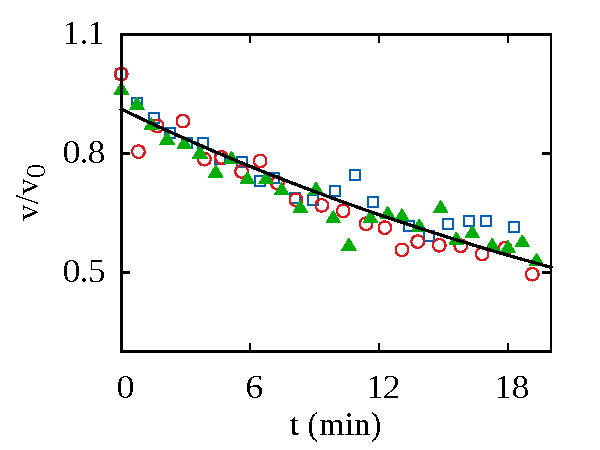
\includegraphics[width=\linewidth]{lifetime.pdf}
    \end{center}
    \caption{Normalized Cboat speed vs. time, fit to $\mathrm{e}^{-\frac{t}{\tau}}$ where $\tau$ represents the life time of a cboat. Symbols correspond to different experimental trials.}
    \label{fig:lifetime}
\end{figure}


%\subsubsection{Oscillatory Motion of the cboat}
%\label{sec:oscboat}
\begin{figure*}[ht]
	\centering
	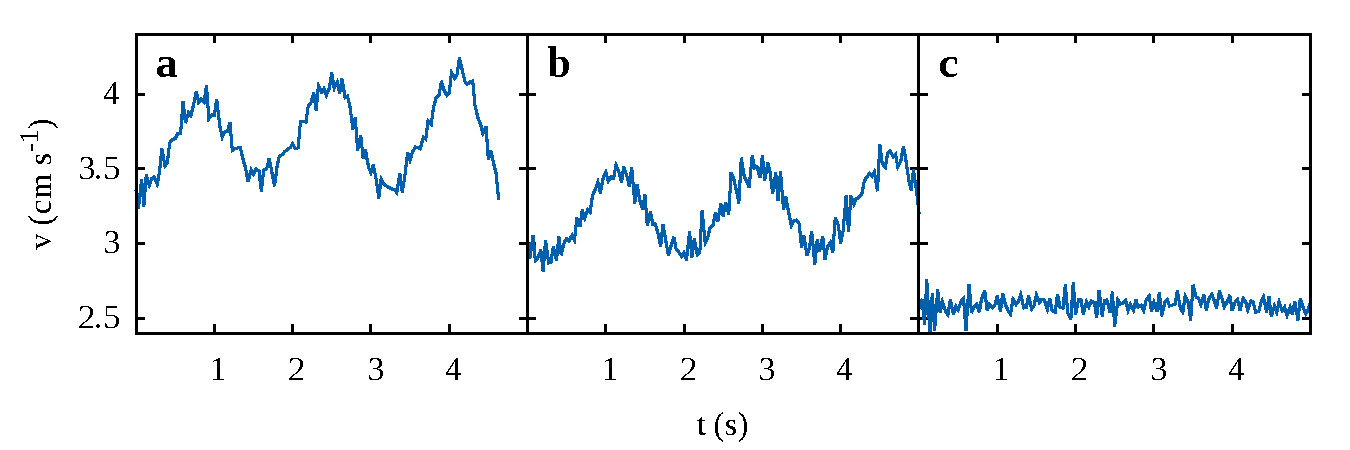
\includegraphics[width=\textwidth]{uvst_72dypcm.pdf}
	\caption{{\bf (a)} at $\sim 4\ \mathrm{min}$, {\bf (b)} at $\sim 7\ \mathrm{min}$, {\bf (c)} at $\sim 16\ \mathrm{min}$}
\label{fig:uvst_72dypcm}
\end{figure*}

With decreasing marangoni force strength in time, the c-boat exhibits three distinct modes of motion over 1-10 s timescales.  Figure~\ref{fig2} also shows time traces of c-boat speed at specific intervals corresponding to these three modes. At early times and high surface tension difference, the c-boat speed exhibits harmonic oscillations about the mean (see fig.~\ref{fig2}b). This mean speed and oscillation amplitude continuously decrease with time {\bf Sathish to confirm, else remove} and transition to the second distinct mode where the c-boat moves with steady speed (see fig.~\ref{fig2}c). The third distinct mode of relaxation oscillations emerges at long times and low surface tension differences where c-boat motion occurs in periodic bursts interspersed with durations where no c-boat motion occurs (see fig.~\ref{fig2}d).

We analysed the amplitude and frequency dependence of the c-boat speed oscillations with time to characterise the behavior within, and the transition between, the individual modes of motion. The amplitude, defined as the difference between the maximum and minimum speed within an oscillation, is plotted in fig.~\ref{fig3}a as a function of time, and the corresponding oscillation frequency is shown in fig.~\ref{fig3}b. The oscillation amplitude in the harmonic regime continuously decreases with time. The instance when the amplitude becomes zero marks the transition to steady motion {\bf (Sathish, approx. and exactly what time?)}. Under the regime of steady motion, the amplitude of oscillations is zero, and the frequency is undefined. At a later time {\bf (Sathish, approx. and exactly what time?)}, the amplitude and the frequency jump to finite values, as the behavior of the cboat transitions to that of relaxation oscillations. The frequency of oscillation after this transition is finite, and continuously decreases with time, whereas the amplitude increases (does it? ... confirm).  Knowing that the Marangoni force strength monotonically decreases with time, the observation that the transitions between the different modes occur at finite times indicates that they occur at a critical value of Marangoni force strength. 

The continuity of the Marangoni force strength with time can be confirmed via visualization of the comet trail left behind the cboat. In particular, the comet trail provides a visualization of the asymmetry in the CA distribution around the cboat. The shape and size of the comet trail is, therefore, indicative of the nature of underlying dynamics, and any abrupt changes would be made visible by the comet trail. Direct visualization of the comet trail for the three modes of cboat motion is shown in fig.~\ref{fig2}e-g. The reducing size of the comet trail implies a decrease in the strength of the net Marangoni force propelling the cboat. {\bf What the hell do we see in the comet trail dynamics?}

To further verify that the Marangoni force strength is indeed the parameter governing these transitions, we independently change the ambient surface tension. By introducing different amounts of SDS in the petri dish, the surface tension was reduced from 72 dy/cm (pure water) down to 59 dy/cm. The motion of  freshly prepared cboats was observed a fixed duration (XX mins) after beginning the experiment, to control for the effects of CA depletion. The cboat in the presence of SDS exhibited the three modes of motion in the same order as the ambient surface tension is continuously decreased. As the time traces of cboat speed in figure 4 show, the cboat motion shows harmonic oscillations for ambient surface tension value of 72 dy/cm, steady motion for XX dy/cm, and relaxation oscillations for 65 dy/cm. The comet tail structure also shows features similar to the those observed when the transitions were a result of CA depletion from the cboat. While introduction of SDS may change the Marangoni forces on the interface, our observations suggest that the qualitative behavior of the cboat motion is preserved under these dynamics.

However, we varied $\xi$ by modifying the air-water interfacial tension using SDS. Figure~\ref{fig:uvst_65dypcm} shows the speed traces of a cboat at different intervals of time when the air-water interfacial tension is lowered to $65\ \mathrm{dy\cdot cm^{-1}}$. We observe that, the average speed of the cboat at different intervals decreases and the period of the oscillations increases. Another subtle observation is the distance travelled by the cboat, area under the speed vs. time curves, between oscillations is approximately equals to the distance, $R$ out to which CA molecules are spread by the Marangoni flow and beyond $R$, CA concentration is zero due to dissolution. During the course of experiment $R$ constantly decreases due to dissolution of CA in water. 
\begin{figure}[ht] 
    \centering
       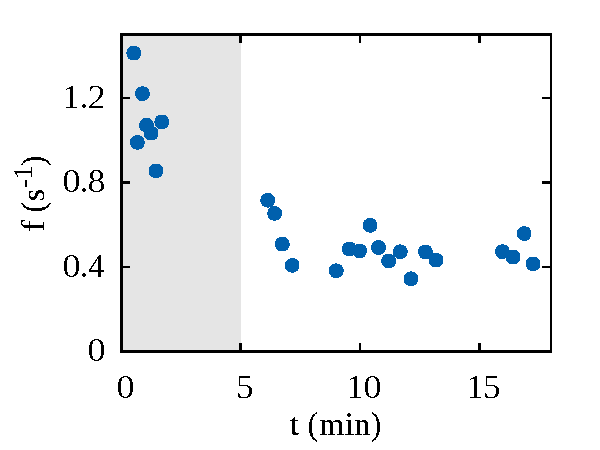
\includegraphics[width=\linewidth]{freqvst.pdf}
    \caption{Frequency of oscillation vs. time. Grayed out area is the transient phase during which excess CA present on the surface of the cboat.}
    \label{fig:freqvst}
\end{figure}
\begin{figure*}[ht]
	\centering
	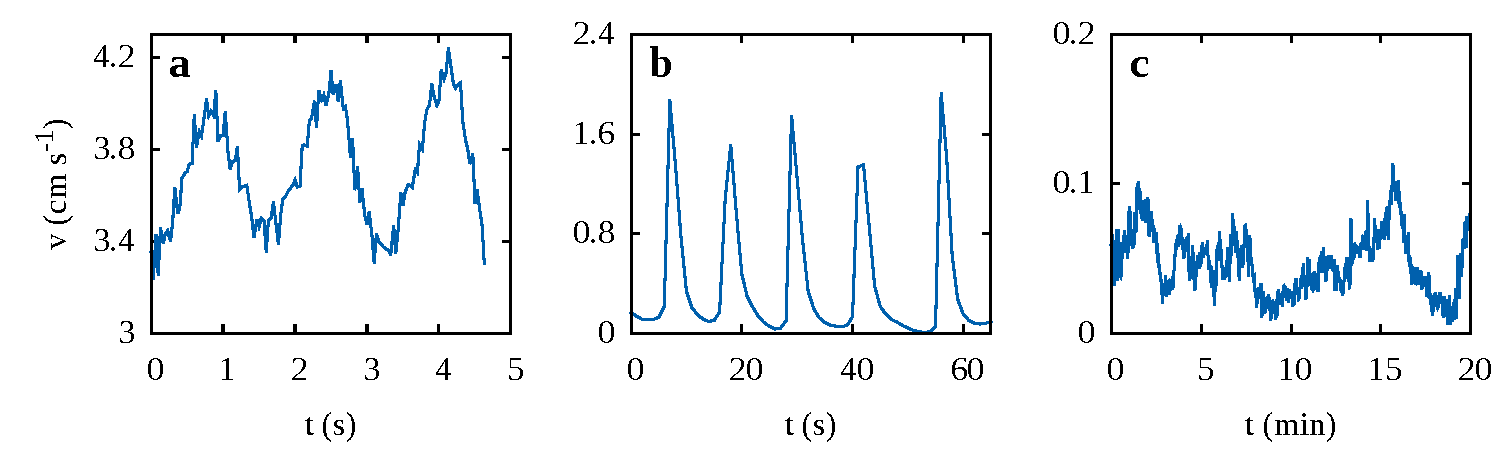
\includegraphics[width=\textwidth]{uvst_sigma.pdf}
	\caption{{\bf (a)} at $\sigma = 72\ \mathrm{dy\ cm^{-1}}$, {\bf (b)} at $\sigma = 65\ \mathrm{dy\ cm^{-1}}$, {\bf (c)} at $\sigma = 59\ \mathrm{dy\ cm^{-1}}$}
\label{fig:uvst_sigma}
\end{figure*}

\section{Summary}
\label{sec:summary}
TBD

\begin{acknowledgement}
VSA, DKS, and MMB were supported by the Collective Interactions Unit at the Okinawa Institute of Science and Technology. MMB acknowledges L. Mahadevan for introducing the camphor boat system and subsequent scientific discussions, and D. Vu Anh for help with preliminary experiments. VSA would like to thank Pinaki Chakraborty for discussions. The authors acknowledge Kenneth J. Meacham III for help with experiments.
\end{acknowledgement}

% \begin{suppinfo}

% This will usually read something like: ``Experimental procedures and
% characterization data for all new compounds. The class will
% automatically add a sentence pointing to the information on-line:

% \end{suppinfo}

% The appropriate \bibliography command should be placed here.
% Notice that the class file automatically sets \bibliographystyle
% and also names the section correctly.

\bibliography{CBoat}
\end{document}
